\documentclass[manuscript,screen,nonacm]{acmart}
\usepackage{booktabs}
\usepackage{graphicx}
\setcopyright{none}
\settopmatter{printacmref=false}
\renewcommand\footnotetextcopyrightpermission[1]{}
\acmDOI{}
\acmISBN{}
\title{RevocationBench: A Local Fault-Injection Pilot for Delegated Agent Authority}
\author{Saurav K. Aryal}
\affiliation{\institution{Howard University}\city{Washington, DC}\country{USA}}
\renewcommand{\shortauthors}{Saurav K. Aryal}
\begin{document}
\begin{abstract}
Delegated tool authority can fail when a permission check and its consequential effect observe different state. We present a small, reproducible integration pilot that measures committed effects under four authored concurrent schedules: competing requests against a shared budget, an authorized within-budget control, repeated operation identifiers, and parent-grant revocation. Two worker threads use separate real SQLite connections. A deliberately weak controller caches a preflight decision; a reference gateway rechecks the grant chain, budget, and operation identifier inside the same transaction that records the local effect. Across 80 related schedules per controller, the weak controller violates at least one invariant in 60 schedules and matches authorized completion in 20; the gateway has zero observed violations and matches authorized completion in all 80. A separate response-loss control produces two external effects under naive retry, versus one effect and one charged unresolved operation under conservative retry suppression. These results validate the measurement harness and a narrow local transaction boundary. They do not establish security for model-driven agents, distributed services, Cedar policies, or arbitrary external endpoints. We describe the stronger comparisons and failure semantics needed for that next study.
\end{abstract}
\keywords{agent authorization, delegation, revocation, fault injection, SQLite, committed effects}
\maketitle

\section{Introduction and Background}
An agent authorized to use a tool may run concurrently with another worker, retry a request after losing its response, or continue after an ancestor grant has been revoked. Evaluating only a tool-call permission decision leaves a practical question unanswered: what actually committed after the decision? A useful evaluation must distinguish an authorized request, a successful effect, a repeated effect, an acknowledged revocation, and an unresolved outcome. It must also check useful completion, because blocking every request would otherwise look secure.

This paper reports an initial engineering pilot for that evaluation. Its setting is intentionally small: one machine, two workers, one local authoritative ledger, and four forced schedule templates. The contribution is an auditable test artifact connecting explicit execution assumptions to database effects. The gateway is a reference implementation of familiar transactional checks, rather than a new authorization language or a new distributed protocol. The study asks three bounded questions. Can the harness expose an authorization check that becomes stale before execution? Does the transactional reference preserve authorized local work while avoiding the seeded violations? What remains unresolved when an effect commits outside its transaction boundary?

AgentDojo provides an extensible environment for tool-using agent tasks and prompt-injection evaluation, including measurements of legitimate task performance and adversarial outcomes~\cite{debenedetti2024agentdojo}. Progent controls agent tool names and arguments using symbolic policies and deterministic checks; its revised design also constrains policy updates~\cite{shi2025progent}. These systems motivate comparisons involving capable agents, but the present experiment executes Python workers without an LLM. It therefore cannot estimate an agent attack-success rate or compare its controller against either system.

Cedar separates policy evaluation from application code and supports policy validation and formal reasoning~\cite{cutler2024cedar}. Its policy semantics are relevant to the next implementation stage. A policy engine is not included in this pilot, and we do not attribute its guarantees to our Python grant lookup. Similarly, the experimental bounded-capability-receipts Internet-Draft explicitly treats shared budgets, replay resistance, and ambiguous external effects as state-management concerns~\cite{schrock2026bounded}. That document is work in progress, not an adopted standard. These ideas are prior art; our proposed research direction is reproducible effect-level testing under execution faults.

\section{Methods}
\subsection{State, mediation, and controllers}
Each trial starts with a fresh SQLite database in write-ahead-log mode. It contains a root grant, a child referring to that root, a budget account with used amount zero and cap 100, a committed-effect table, and an operation table. Workers always request the child grant. Both workers establish their own database connections and read the account and child status before waiting at a barrier. A coordinator joins the barrier, optionally commits a root revocation, and releases both workers. Per-worker jitter is sampled uniformly between zero and two milliseconds using a fixed seed. The 20 replicates use seeds 2026--2045. They vary worker timing within the same four templates; they are not 80 distinct workflows.

The \emph{cached-preflight} baseline checks the child grant and budget before the barrier. After release it trusts that cached decision, starts an immediate transaction, writes the account as its previously observed amount plus the requested amount, and inserts an effect. It does not recheck the parent, reserve a shared budget against current state, or reject duplicate operation identifiers. This baseline is deliberately weak. Its account update can lose another worker's update; consequently, the account field alone can understate actual spending. It is an integration control rather than a competitive authorization system.

The \emph{transactional gateway} starts an immediate transaction after release. Inside that transaction it first checks whether the operation identifier already exists, reads current budget state, and follows the child-to-root grant chain. A missing, revoked, or cyclic chain is rejected. A new authorized operation atomically increments used budget, records a complete operation, inserts the local effect, and commits. An existing identifier causes no second effect. Exceeding the budget or using a revoked grant rolls the transaction back. All simulated local effects occur in the same database as these checks. This reliance on one serialized writer boundary is consistent with SQLite's documented connection isolation and transaction behavior~\cite{sqliteisolation}; it is also the main limit on transfer to external systems.

\subsection{Schedules and outcomes}
Table~\ref{tab:schedules} specifies all templates and authorized counts. In the budget race, two different operations each request 60 units, so at most one can commit under cap 100. In the within-budget control, distinct requests for 60 and 40 may both commit. In the replay case, two requests share an identifier and amount 40, so exactly one effect is authorized. In the revocation case, distinct requests for 30 are released only after the coordinator commits revocation of their root grant. No resulting effect is authorized.

\begin{table}[t]
\centering
\caption{Authored local schedule templates. Each is run 20 times per controller with two workers. The expected count is a fixture oracle, not an agent-generated judgment.}
\label{tab:schedules}
\begin{tabular}{lrrl}
\toprule
Schedule & Amounts & Expected effects & Injected condition\\
\midrule
Shared budget & 60, 60 & 1 & Both preflights precede release\\
Within-budget control & 60, 40 & 2 & Both preflights precede release\\
Repeated operation & 40, 40 & 1 & Same operation identifier\\
Ancestor revocation & 30, 30 & 0 & Root revoked before release\\
\bottomrule
\end{tabular}
\end{table}

We read the committed effect rows after both workers finish. A trial violates the tested specification if the effect amounts sum to more than 100, an operation identifier has multiple effects, or an effect timestamp follows the acknowledged root revocation. The local acknowledgement timestamp is recorded in the same transaction as the revocation and is compared with a process monotonic clock. It is not a distributed clock or a test of an already-running external action. Authorized-completion matching requires both the expected number of effects and absence of a violation. Worker decisions and latency are preserved for inspection, but only the committed effects determine the primary outcomes.

\subsection{External response-loss control and provenance}
A separate control uses a second SQLite database as an endpoint outside the ledger transaction. Its receipt insert really commits, after which the response is deliberately treated as lost. The naive controller retries once, creating a second receipt. The gateway first records an unknown operation and reserves 40 units in its ledger, then invokes the endpoint. On the second attempt it sees that unresolved identifier and suppresses retry. This is a conservative ambiguity policy, not an implementation of the full capability-receipts draft. It is tested once per controller and is reported separately from the 80 local schedules.

The preserved run contains \texttt{trials.csv}, worker traces, boundary-control JSON, and the underlying databases. The figure generator derives counts directly from the CSV and JSON, cross-checks them against the recorded result, and emits SHA-256 hashes in \texttt{figures/derived\_summary.json}. The archived experiment-module hash is \texttt{fe00c8cd}\ldots\texttt{f631e}; the complete digest is included in the recorded source manifest. The pilot used no model calls. It ran in approximately 0.95 seconds on the recorded arm64 macOS host with Python 3.14.2. This elapsed time describes this tiny integration fixture, not production throughput or an inference cost comparison.

\section{Results}
\subsection{Local effects and useful completion}
The cached-preflight controller violates the tested specification in 60 of 80 schedules. These consist of all 20 budget races, all 20 repeated-identifier schedules, and all 20 ancestor-revocation schedules. The budget race produces 120 units of committed effects in each replicate, for 400 aggregate excess units; its recorded account field nevertheless remains 60. The repeated-identifier schedules produce 20 duplicate effects in aggregate. The revocation schedules produce 40 effects after the acknowledged root revocation. Reporting these effect-level quantities exposes failures that a final budget-account value or a worker's successful return could miss.

The gateway has zero observed violations across its 80 local schedules and matches authorized completion in all 80. The weak baseline matches authorized completion only in the 20 within-budget controls. Both controllers complete both authorized effects in every such control. Thus the gateway's observed safety result in this fixture is accompanied by a positive test of permitted work. Figure~\ref{fig:local} shows the full scenario breakdown rather than a single aggregate percentage.

\begin{figure}[t]
\centering
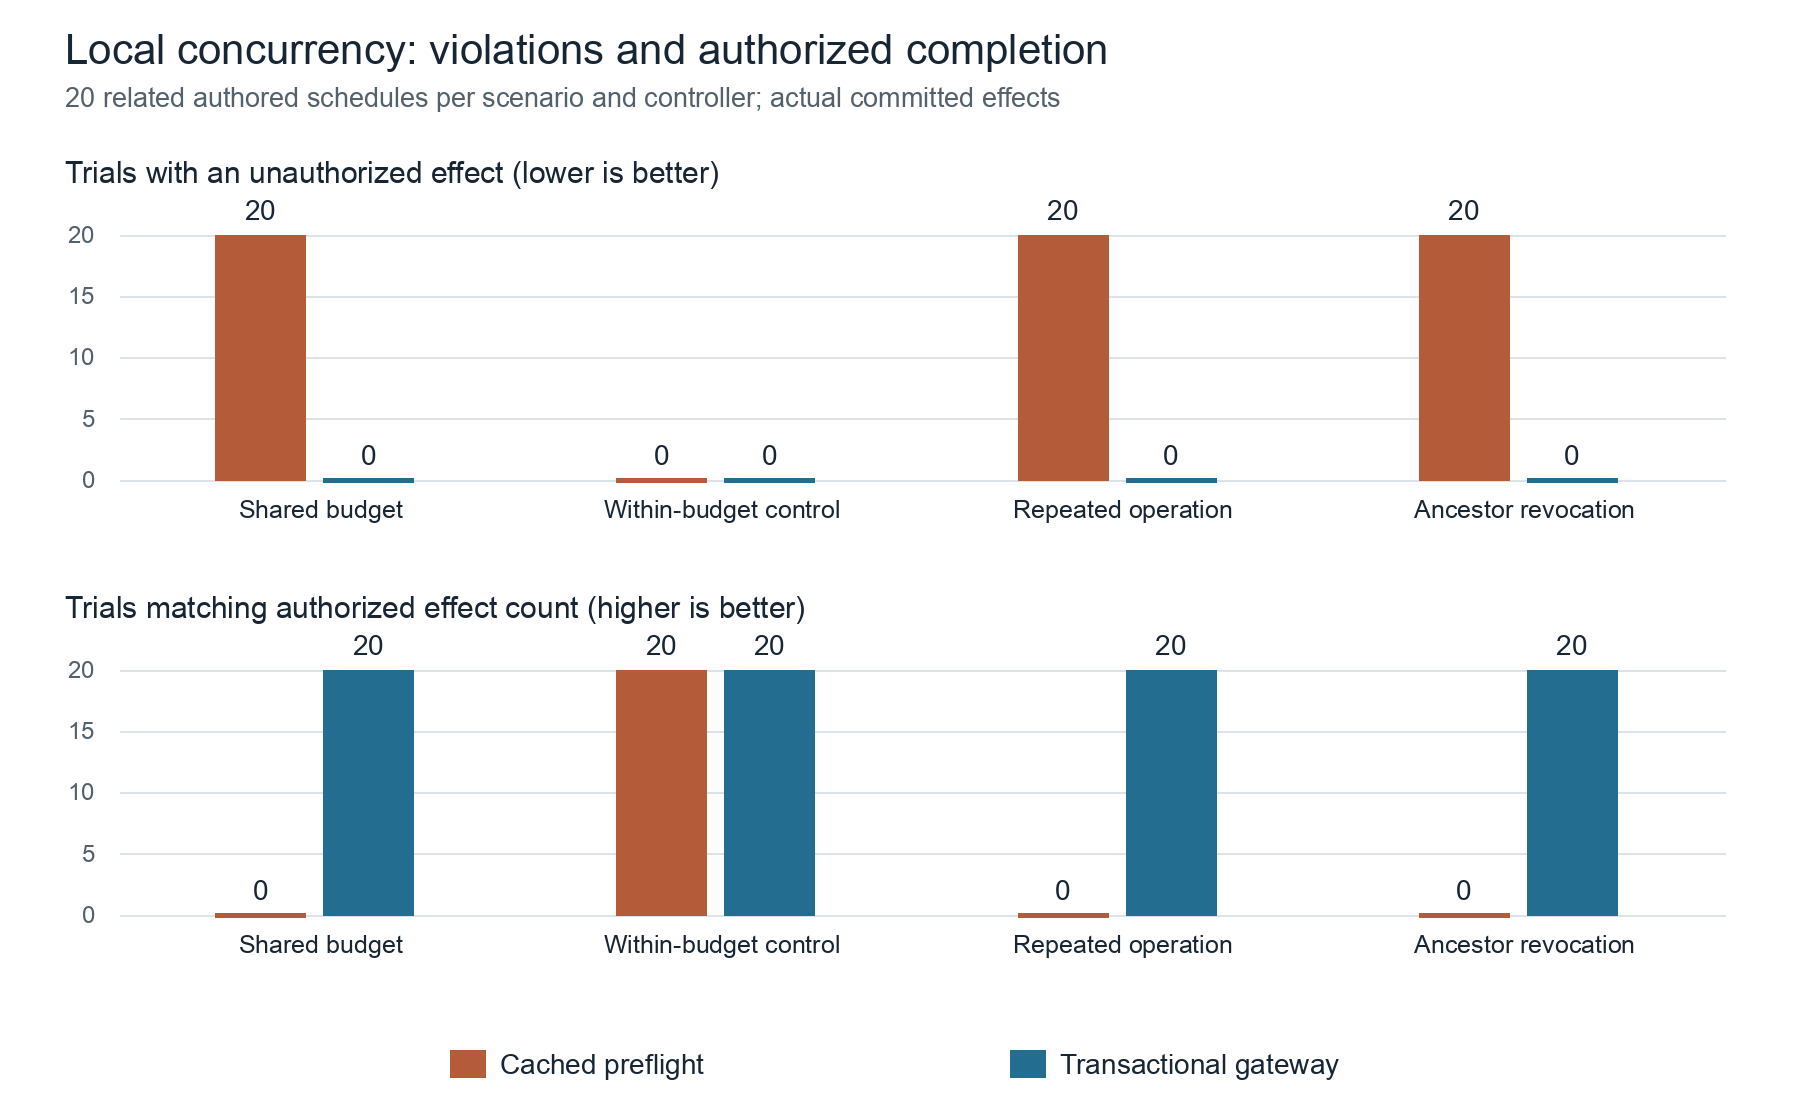
\includegraphics[width=.97\linewidth]{figures/local_results.png}
\caption{Descriptive counts from the preserved local pilot. Each bar has denominator 20. Security and authorized completion are separate outcomes. The related forced schedules do not support population failure-rate estimates.}
\Description{Two bar-chart panels compare cached preflight and the transactional gateway. Preflight has twenty violations in the budget, repeated-operation, and revocation scenarios and zero in the within-budget control. The gateway has zero violations in all four. Authorized-completion matches are zero for preflight in the three fault scenarios and twenty in the control, and twenty for the gateway in every scenario.}
\label{fig:local}
\end{figure}

\subsection{The unresolved external boundary}
Under deliberately lost external responses, naive retry produces two committed endpoint receipts. The gateway produces one receipt, retains one unknown operation, reserves 40 units, and refuses the second attempt. Neither controller confirms task completion. Figure~\ref{fig:boundary} presents this outcome separately because suppressing a duplicate is not equivalent to resolving the original operation. The gateway cannot determine from the missing response whether the endpoint committed; our offline audit can see the receipt, whereas the simulated controller cannot.

\begin{figure}[t]
\centering
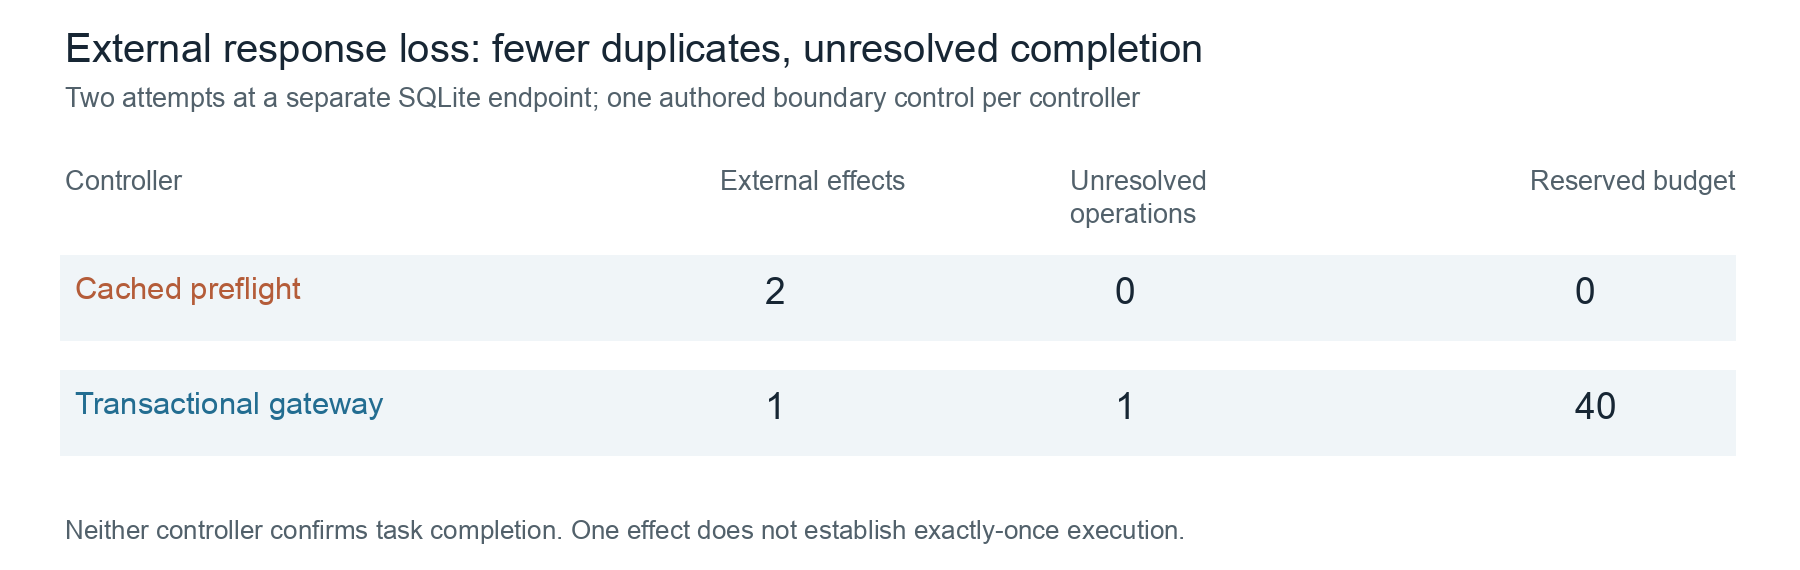
\includegraphics[width=.97\linewidth]{figures/external_boundary.png}
\caption{One external-response-loss control per controller. The gateway avoids the second effect by leaving authority charged and completion unresolved. This is an observed boundary condition, not an exactly-once guarantee for arbitrary endpoints.}
\Description{A table shows cached preflight producing two external effects, zero unresolved ledger operations, and zero reserved budget. The transactional gateway produces one external effect, one unresolved ledger operation, and reserves forty units. Neither confirms completion.}
\label{fig:boundary}
\end{figure}

\subsection{Interpretation and limits}
The local result is expected given the implementation: the reference gateway places the seeded checks and effects inside the same transaction. The useful finding is that the artifact measures those boundaries consistently, detects all three seeded failure modes in its weak control, and retains an explicit authorized-work control and an unresolved-outcome category. It is not evidence that transactional authorization is a new idea or that a sophisticated baseline would fail similarly.

The schedules are authored, timing is forced at one barrier, and repeated trials share their application schema and threat template. We therefore report counts without binomial confidence intervals or a claim that zero observations bound a production failure rate. We did not test process crashes, network partitions, multiple authoritative replicas, forged grants, compromised mediation, arbitrary delegation depth, or model-generated tools. Grant authentication and policy grounding are trusted rather than evaluated. Latency includes worker waiting and artificial jitter, so this run does not establish gateway overhead. The separate endpoint experiment does not test an idempotent endpoint or a reconciliation service; those stronger alternatives could change the ambiguity tradeoff.

\section{Future Work}
The next study should replace the cached-preflight integration control with stronger, clearly specified systems: a transactionally correct ledger without ancestor propagation, a policy-only gateway, and a gateway with durable operation identifiers and endpoint reconciliation. Ablations should isolate parent revocation, shared-budget accounting, and duplicate suppression rather than credit their bundled implementation to a single mechanism. Each backend must state its authority domain and the point at which a revocation acknowledgement becomes enforceable. Claims for in-flight operations need their own cancellation and reconciliation semantics.

A practical one-year extension would connect real tool-using agents to a small set of instrumented workflows, including purchases, document access, and delegated administrative changes. The benchmark would preserve benign completion tasks alongside prompt-injection and execution-fault variants. Cedar can provide a separately tested policy-decision component; it should not be presented as solving ledger atomicity. AgentDojo-style tasks and Progent-style privilege controls offer relevant starting points for agent utility and enforcement comparisons. Integrations should use their released implementations and document any modifications before a held-out evaluation.

Execution faults should then cross process and service boundaries: a crash before admission, after a reservation, after an endpoint effect, and before its response; concurrent retries; delayed revocation delivery; and stale or duplicated messages. Separate development schedules and locked evaluation families would limit tuning to the benchmark. Tests should include idempotent and non-idempotent endpoints, reconciliation delays, and legitimate retries after a proven no-effect outcome. The primary frontier would report committed unauthorized effects, authorized completion, unresolved charged operations, recovery time, and resource cost together. This would make the cost of conservative uncertainty visible instead of treating every blocked retry as a success.

\section{Conclusion}
This pilot supports a narrow feasibility claim: a small effect-audited harness can expose seeded budget, replay, and ancestor-revocation races while checking permitted local completion. Its transactional reference meets all 80 authored local schedules. Its separate endpoint control also makes the limitation concrete: one external effect remains charged and unresolved after response loss. Moving from this integration result to agent security requires capable agents, stronger baselines, explicit distributed semantics, and held-out fault families.

\paragraph{Artifact and author statement.}
The paper package includes the observed tables, figure-generation code, source digests, and a reproduction guide. The artifact repository is \url{https://github.com/Saurav-K-Aryal/revocationbench-pilot}. Saurav K. Aryal is the sole listed author and executor of the preliminary experiments. AI assistance was used for code, analysis, and manuscript drafting under the author's direction; this draft requires the author's review before submission.

\bibliographystyle{ACM-Reference-Format}
\bibliography{refs}
\end{document}
